\documentclass[10pt]{article}
\usepackage{amsfonts}
\usepackage{fancyhdr}
\usepackage{comment}
\usepackage[letterpaper, top=2.5cm, bottom=2.5cm, left=2.2cm, right=2.2cm]%
{geometry}
\usepackage{amsmath}
\usepackage{subfig}
\usepackage{mathtools}
\usepackage{changepage}
\usepackage{enumitem}
\usepackage{amssymb}
\usepackage{graphicx}
\usepackage{hyperref}
\usepackage{listings}
\usepackage{color}
\usepackage{textcomp}
\usepackage{courier}

\definecolor{listinggray}{gray}{0.9}
\definecolor{lbcolor}{rgb}{0.96,0.96,0.96}
\lstset{
    backgroundcolor=\color{lbcolor},
    tabsize=4,
    rulecolor=,
    language=Python,
        basicstyle=\footnotesize\ttfamily,
        upquote=true,
        aboveskip={1.0\baselineskip},
        columns=fixed,
        extendedchars=true,
        breaklines=true,
        prebreak = \raisebox{0ex}[0ex][0ex]{\ensuremath{\hookleftarrow}},
        frame=single,
        showtabs=false,
        showspaces=false,
        showstringspaces=false,
        identifierstyle=\ttfamily,
        keywordstyle=\color[rgb]{0,0,1},
        commentstyle=\color[rgb]{0.133,0.545,0.133},
        stringstyle=\color[rgb]{0.627,0.126,0.941},
}

\newcommand{\by}{\mathbf{y}}

\begin{document}

    \title{SDS 383D, Exercises 3: Linear smoothing and Gaussian processes}
    \author{Tyler Buffington}
    \date{\today}
    \maketitle

    \section*{Curve fitting by linear smoothing}
    \begin{enumerate}[label=(\Alph*)]
    \item
    
    We begin with the linear regression equation:
    $$y_i = \beta x_i + \epsilon_i$$
       
    Recall that we derived the least-squares estimator for multiple regression:

    $$\hat{\beta} = (X^TX)^{-1}X^Ty$$

    For the case with the means subtracted, this is equivalent to 
        
    $$\frac{\sum_{i=1}^{n}x_iy_i}{\sum_{i=1}^{n}x_i^2}$$

    Back to our regression equation for one value, but for an new point, $x^*$

    $$\hat{y}^* = \hat{\beta}x^*$$

    Note that the error term is excluded because it has mean zero. Substituting in what we derived for $\hat{\beta}$:
    $$\hat{y^*} =\frac{\sum_{i=1}^{n}x_iy_i}{\sum_{i=1}^{n}x_i^2}x^*$$

    which can then be written like:

    $$\hat{y}^* = \sum_{i=1}^{n}w(x_i,x^*)y_i$$
    where
    $$w(x_i,x^*)= \frac{x_ix^*}{\sum_{j=1}^{n}x_j^2}$$
    This smoothes the data by collapsing it to the least-squares regression line. The K-nearest-neighbor smoothing will conversely take the average of the K nearest points (by x). It is worth noting that in the linear smoother, data points with x values very far away from $\bar{x}$ are assigned large weights.	

    \item
    The code for the analysis can be found in kernel\_smooth.py. The resulting plot is shown below: 
    \begin{figure}[htb] \centering
    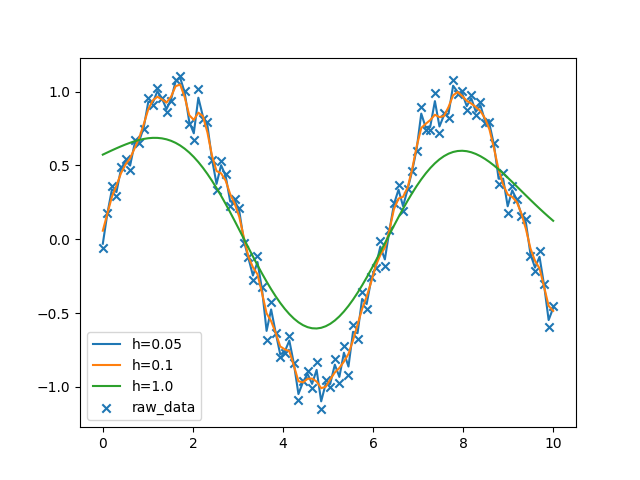
\includegraphics[width=0.95\textwidth]{./gaussian_kernel.png}
    \caption{The fit for different bandwidth values.}
    \label{fig:gaussian_kernel}
    \end{figure}
    
    This plot illustrates the bias-variance tradeoff: as h increases, the fit becomes less noisy, but more biased. In the limit as h goes to $\inf$, the fit becomes a flat line at the mean because this would mean that all points have equal weight. On the other hand, as h goes to zero, the fit would match the data exactly, which is also not useful because it would pick up the noise from the raw data as well.
	\end{enumerate}

    \section*{Cross validation}
    \begin{enumerate}[label=(\Alph*)]
    \item
    See cross\_validaiton.py.
    \item
    The methodology is detailed in bandwidth\_select.py. The smooth function was chosen to be $y=x^3$ and tthe wiggly function was chosen to be $y=sin(50x)$. The error as a function of bandwidth, h, is plotted below:

    \begin{figure}[htb] \centering
    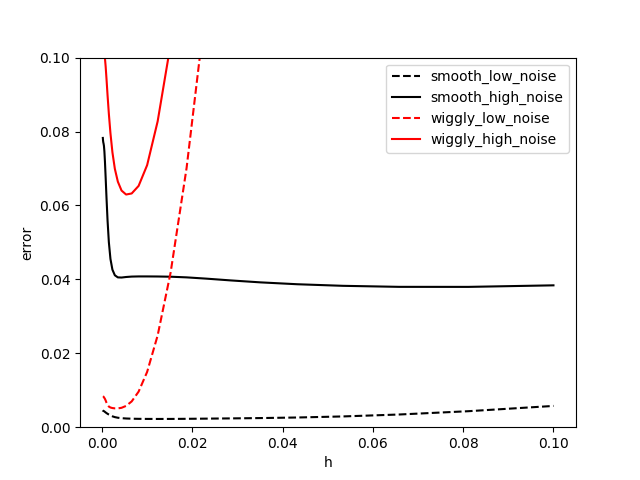
\includegraphics[width=0.95\textwidth]{./h_select.png}
    \caption{the error for different bandwidth values.}
    \label{fig:h_select}
    \end{figure}

    the main features are that the noisy functions have higher errors at the optimal h, and the noise also increases the value for the optimal h. the optimal fits are shown for the four cases below in Figure \ref{fig:results}

    \begin{figure}[!b]
    \begin{center}
    %
    \subfloat[smooth low noise]{%
      \label{fig:sl} 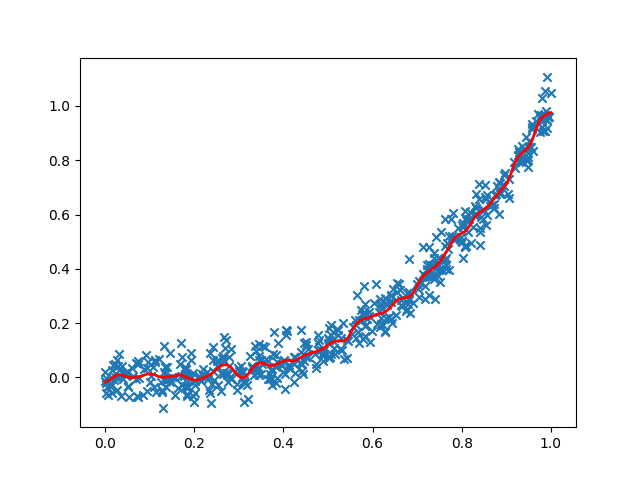
\includegraphics[width=7cm,keepaspectratio]{./smooth_low_noise.png}
    }%
    \subfloat[smooth high noise]{%
     \label{fig:sh} 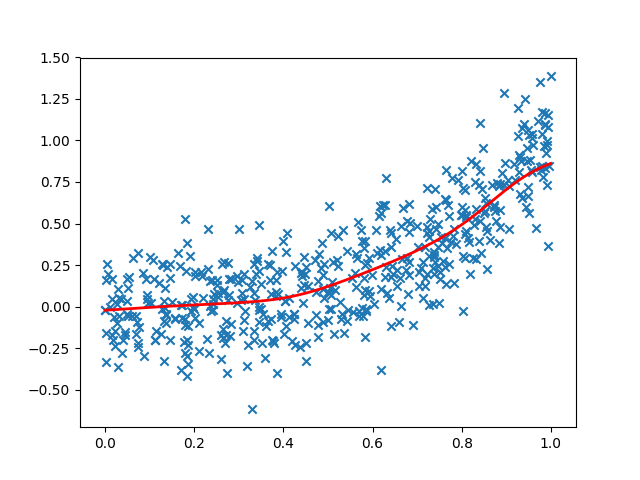
\includegraphics[width=7cm,keepaspectratio]{./smooth_high_noise.png}
    }\\ %  ------- end of the first row ----------------------%
    \subfloat[wiggly low noise]{%
      \label{fig:wl} 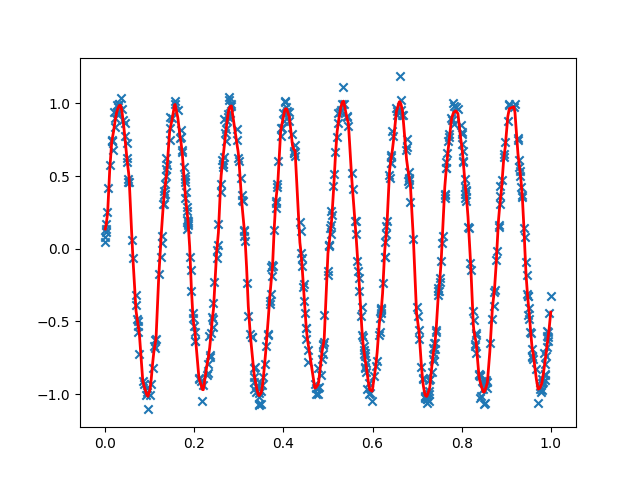
\includegraphics[width=7cm,keepaspectratio]{./wiggly_low_noise.png}
    }%
    \subfloat[wiggly high noise]{%
     \label{fig:wh} 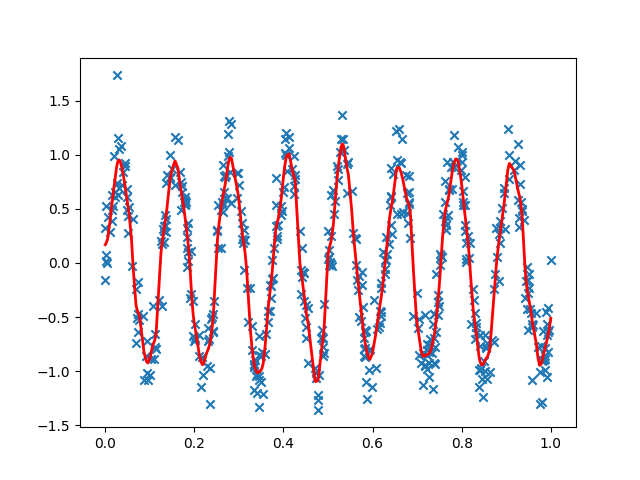
\includegraphics[width=7cm,keepaspectratio]{./wiggly_high_noise.png}
    }\\ %  ------- end of the second row ----------------------%

    \end{center}
    \caption{The fits at the optimal h for the four cases.}
    \label{fig:results}
    \end{figure}
    \clearpage
    \end{enumerate}
    \section*{Local polynomial regression}
        \begin{enumerate}[label=(\Alph*)]
        \item

        For points u in a neighborhood of the target point x, define the polynomial
        $$g_x(u;a) = a_0 + \sum_{k=1}^Da_k(u-x)^k$$
        where 
        $$\hat{a} = \arg \min_{R^{D+1}}  \sum_{i=1}^{n}w_i\{y_i-g_x(x_i;a)\}^2$$
        substitute in $g_x(x_i;a)$

        $$\hat{a} = \arg \min_{R^{D+1}}  \sum_{i=1}^{n}w_i\{y_i-a_0 - \sum_{k=1}^Da_k(x_i-x)^k\}^2$$
        Then define matrix R such that $R_{i,j} = (x_i-x)^{j-1}$, so then we get 

        $$\hat{a} = \arg \min_{R^{D+1}}  \sum_{i=1}^{n}w_i\{y_i-Ra\}^2$$
        If we define W to be a diagonal matrix where $W_{i,i}=w_i$, and all off diagonal terms are zero, we get

        $$\hat{a} = \arg \min_{R^{D+1}}  \{y-Ra\}^TW\{y-Ra\}$$
        Then evaluate derivative and set equal to zero to minimize:

        $$\frac{d}{da}\{y-Ra\}^TW\{y-Ra\}$$
        $$=\frac{d}{da}[y^TWy-2y^TWRa+a^TR^TWRa]$$
        $$=-2R^TWy+2R^TWRa = 0$$
        $$R^TWRa=R^TWy$$
        $$a = (R^TWR)^{-1}R^TWy$$
        We can then define a matrix $M=(R^TWR)^{-1}W$ so that we get the final clean form:
        $$a=My$$
        \item
        Beginning with result from part A:
        $$a = (R^TWR)^{-1}R^TWy$$


        $$=\Bigg(
        \begin{bmatrix}
        1 & \dots & 1 \\ 
        (x_1-x) & \dots & (x_n-x)
        \end{bmatrix}
        \begin{bmatrix} 
        w_1 & \dots & 0 \\ 
        \vdots & \ddots & \vdots \\ 
        0 & \dots & w_n 
        \end{bmatrix}
        \begin{bmatrix}1&(x_1-x)\\ 
        \vdots & \vdots \\ 
        1 & (x_n - x) \end{bmatrix}
        \Bigg)^{-1}
        \begin{bmatrix} 
        w_1 & \dots & 0 \\ 
        \vdots & \ddots & \vdots \\ 
        0 & \dots & w_n 
        \end{bmatrix}
        \begin{bmatrix} 
        1 &(x_1-x) \\ 
        \vdots & \vdots \\ 
        1 & (x_n - x) \end{bmatrix}
        \begin{bmatrix}
        y_1\\
        \vdots\\
        y_n
        \end{bmatrix}
        $$

        $$=\begin{bmatrix}
        \sum_{i=1}^nw_i & \sum_{i=1}^{n}w_i(xi-x) \\
        \sum_{i=1}^{n}w_i(x_i-x) & \sum_{i=1}^nw_i(x_i-x)^2
        \end{bmatrix}^{-1}
        \begin{bmatrix}
        \sum_{i=1}^{n}y_iw_i \\
        \sum_{i=1}^n y_iw_i(x_i-x)
        \end{bmatrix}$$

        $$=\frac{1}{\sum_{i=1}^nw_i \sum_{i=1}^nw_i(x_i-x)^2 - (\sum_{i=1}^nw_i (x_i-x))^2}
        \begin{bmatrix}
        \sum_{i=1}^nw_i(x_i-x)^2 & -\sum_{i=1}^{n}w_i(x_i-x) \\
        -\sum_{i=1}^{n}w_i(x_i-x) & \sum_{i=1}^nw_i     
        \end{bmatrix}
        \begin{bmatrix}
        \sum_{i=1}^{n}y_iw_i \\
        \sum_{i=1}^n y_iw_i(x_i-x)
        \end{bmatrix}$$

        $$=\frac{1}{\sum_{i=1}^nw_i \sum_{i=1}^nw_i(x_i-x)^2 - (\sum_{i=1}^nw_i (x_i-x))^2}
        \begin{bmatrix}
        \sum_{i=1}^nw_i(x_i-x)^2\sum_{i=1}^ny_iw_i - \sum_{i=1}^nw_i(x_i-x)\sum_{i=1}^ny_iw_i(x_i-x) \\
        -\sum_{i=1}^nw_i(x_i-x)\sum_{i=1}^ny_iw_i+\sum_{i=1}^nw_i\sum_{i=1}^ny_iw_i(x_i-x)
        \end{bmatrix}$$

        It can be seen that at the target point x, $\hat{f} = a_0$, so we get 
        $$\hat{f} =  \frac{\sum_{i=1}^nw_i(x_i-x)^2\sum_{i=1}^ny_iw_i - \sum_{i=1}^nw_i(x_i-x)\sum_{i=1}^ny_iw_i(x_i-x)}{\sum_{i=1}^nw_i \sum_{i=1}^nw_i(x_i-x)^2 - (\sum_{i=1}^nw_i (x_i-x))^2}$$

        Let $s_1 = \sum_{i=1}^nw_i(x_i-x)$ and $s_2 = \sum_{i=1}^nw_i(x_i-x)^2$. So then we get:

        $$\hat{f} = \frac{s_2\sum_{i=1}^ny_iw_i-s_1\sum_{i=1}^ny_iw_i(x_i-x)}{\sum_{i=1}^nw_is_2 - s_1\sum_{i=1}\textbf{}^nw_i(x_i-x)}$$

        $$= \frac{\sum_{i=1}^ny_iw_i\big(s_2-s_1(x_i-x)\big)}{\sum_{i=1}^nw_i\big(s_2-s_1(x_i-x)\big)}$$

        Define $w_i^* = w_i\big(s_2 - s_1(x_i-x)\big)$, so then we get the desired form:
        $$\hat{f} = \frac{\sum_{i=1}^nw_i^*y_i}{\sum_{i=1}^nw_i^*}$$
        \item
        Let $q^T=[1,0...0]M$ so that $\hat{f}(x)=a_0=q^Ty$ First find the mean, 
        $$E\big(\hat{f}(x)\big) = E\big(q^Ty\big)$$
        $$=q^T E\big(y\big)$$
        $$ = q^Tf(x)$$
        Then find the variance (remembering the formula for linear transforms):
        $$var(\hat{f}(x) = var(q^Ty)$$
        $$=var\big(q^Tvar(y)q\big)$$
        $$=q^T\sigma^2Iq$$
        $$=\sigma^2q^Tq$$

        \item
        Begin with given equation:
        $$E(\hat{\sigma}) = E\bigg(\frac{||r||_2^2}{n-2tr(H)+tr(H^TH)}\bigg)$$
        $$=\frac{E\bigg[ (y-Hy)^T(y-Hy) \bigg]}{n-2tr(H)+tr(H^TH)}$$
        $$=\frac{E\bigg[y^Ty-2y^TH^T+y^TH^THy\bigg]}{n-2tr(H)+tr(H^TH)}$$
        Then by linearity:
        $$=\frac{E\bigg[y^Ty\bigg]-E\bigg[2y^TH^T\bigg]+E\bigg[y^TH^THy\bigg]}{n-2tr(H)+tr(H^TH)}$$
        Then using the given equation, this reduces to:
        $$=\frac{tr(I\sigma^2)+f^T(x)f(x)--2\bigg(tr(H\sigma^2)+f^T(x)Hf(x)\bigg)+tr(H^TH\sigma^2)+f^T(x)H^THf(x)}{n-2tr(H)+tr(H^TH)}$$

        $$=\frac{n\sigma^2+f^T(x)f(x)--2\bigg(tr(H\sigma^2)+f^T(x)Hf(x)\bigg)+tr(H^TH\sigma^2)+f^T(x)H^THf(x)}{n-2tr(H)+tr(H^TH)}$$

        Factoring out $\sigma^2$:
        $$=\frac{\sigma^2\bigg(n-2tr(H) + tr(H^TH)\bigg) + f^T(x)f(x) +2f^T(x)Hf(x)+f^T(x)H^THf(x)}{n-2tr(H)+tr(H^TH)}$$

        $$=\sigma^2 + \frac{\bigg(f(x)+H(x)f(x)\bigg)^T\bigg(f(x)+H(x)f(x)\bigg)}{n-2tr(H)+tr(H^TH)}$$

        $$=\underbrace{\sigma^2}_{I} + \underbrace{\frac{||f(x)+H(x)f(x)||}{n-2tr(H)+tr(H^TH)}}_{II}$$


        Term $I$ represents the variance and term $II$ represents the bias. Therefore, to reduce the bias, one can simple increase the sample size (n).

        \item
        The relevant code can be found in "local\_linear\_estimator.py"

        \item
     	The residuals are plotted below in Figure \ref{fig:residual_plot}
		\begin{figure}[htb] \centering
		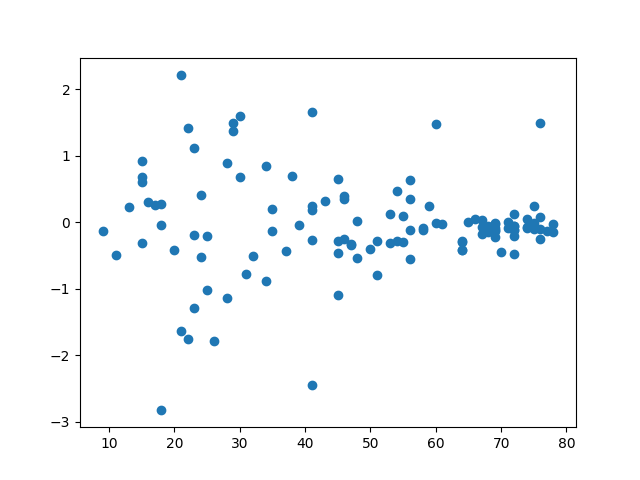
\includegraphics[width=0.95\textwidth]{./residual_plot.png}
		\caption{A plot of the residuals vs. x}
		\label{fig:residual_plot}
		\end{figure}

		The residuals seem to get smaller as x increases, which indicates a lack of homoskedacity.

		\item
		The plot with the confidence bands is shown below in Figure \
     	The residuals are plotted below in Figure \ref{fig:local_linear_estimate}
		\begin{figure}[htb] \centering
		
\includegraphics[width=0.95\textwidth]{./local_estimate.png}
		\caption{The plot of the fit with confidence bands}
		\label{fig:local_linear_estimate}
		\end{figure}

	\end{enumerate}
		\section{Gaussian processes}
        \begin{enumerate}[label=(\Alph*)]
        \item This code is in gaussian\_process.py
        In order to gain an intuition for the effect of each hyperparameter, I established a base case in which $b, \tau_1^2$, and $\tau_2^2$ were all set to $10^-6$. The resulting function is shown in Figure \ref{fig:base_case}. I also made plots in which each hyperparameter is increased to $10^-3$ to examine the effects of each. These are shown in Figures \ref{fig:increased_b}, \ref{fig:increased_tau1}, and \ref{fig:increased_tau2}. The effect of increasing the bandwidth, b, is that is slightly smooths the function as expected. Increasing $\tau_1^2$ also serves to smooth the function because it amplifies the off-diagonal covariance terms. Converesly, increasing $\tau_2^2$ makes the function more noisy because it increases the on-diagonal covariance terms. 
        
        
        \begin{figure}[htb] \centering
        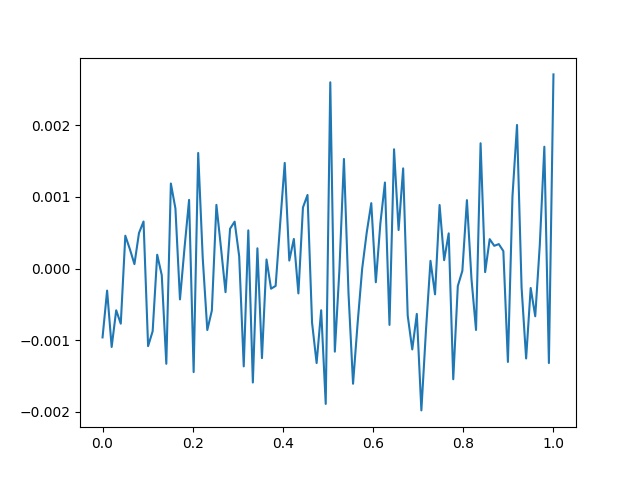
\includegraphics[width=0.95\textwidth]{./base_case.png}
        \caption{The base case from the matern covariance function}
        \label{fig:base_case}
        \end{figure}
        
        \begin{figure}[htb] \centering
        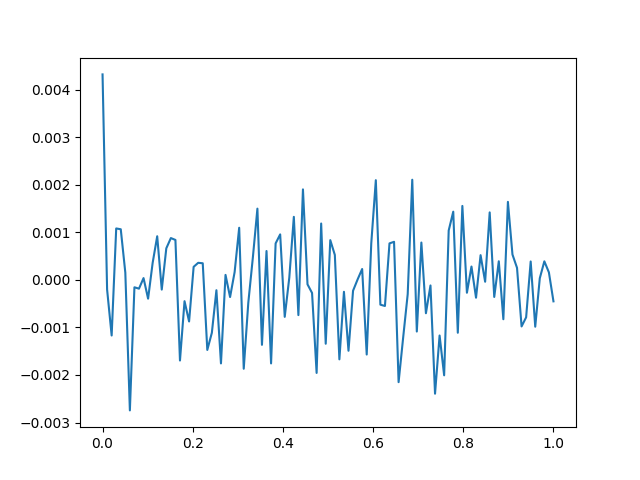
\includegraphics[width=0.95\textwidth]{./increased_b.png}
        \caption{the case with b increased to  0.001}
        \label{fig:increased_b}
        \end{figure}
        
        \begin{figure}[htb] \centering
        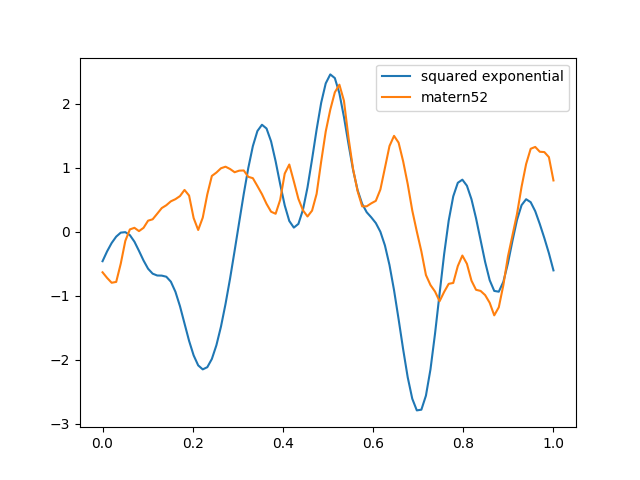
\includegraphics[width=0.95\textwidth]{./increased_tau1.png}
        \caption{The case with $\tau_1$ increased to 0.001}
        \label{fig:increased_tau1}
        \end{figure}
        
        \begin{figure}[htb] \centering
        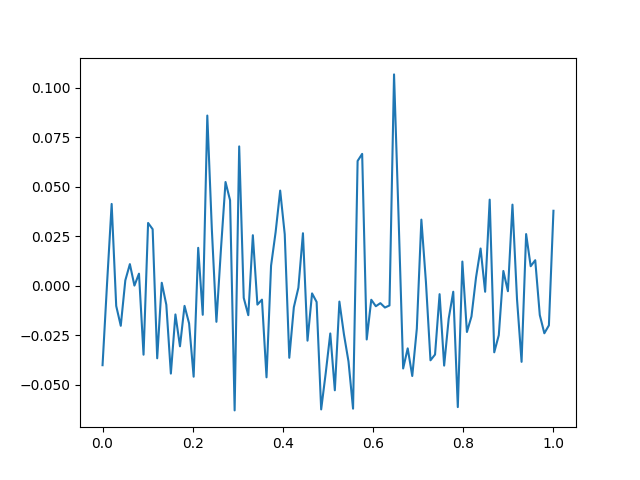
\includegraphics[width=0.95\textwidth]{./increased_tau2.png}
        \caption{The case with $\tau_2$ increased to 0.001}
        \label{fig:increased_tau2}
        \end{figure}
        
        
        
        
        \item
        \item
        We can say that $y = R\theta + N(0,\Sigma)$ and that $\theta = I\theta + 0 N(0,\Sigma)$. We can express the equations like this:


        $$\begin{bmatrix}y \\ \theta \end{bmatrix}
        = \begin{bmatrix} R \\ I \end{bmatrix} \theta
        +\begin{bmatrix} I \\ 0 \end{bmatrix} N(0,\Sigma)$$

        $$=\begin{bmatrix} R & I \\ I & 0 \end{bmatrix}
        \begin{bmatrix} \theta \\ N(0,\Sigma) \end{bmatrix}$$

        Which is just an affine transformation of multivariate normal distributions, therefore, the joint, distribution $p(\big[y,\theta\big]^T)$ is also multivariate normal. 

    \end{enumerate}
\end{document}
\grid
